\documentclass{standalone}
\usepackage{tikz}
\usetikzlibrary{patterns, positioning}


\begin{document}
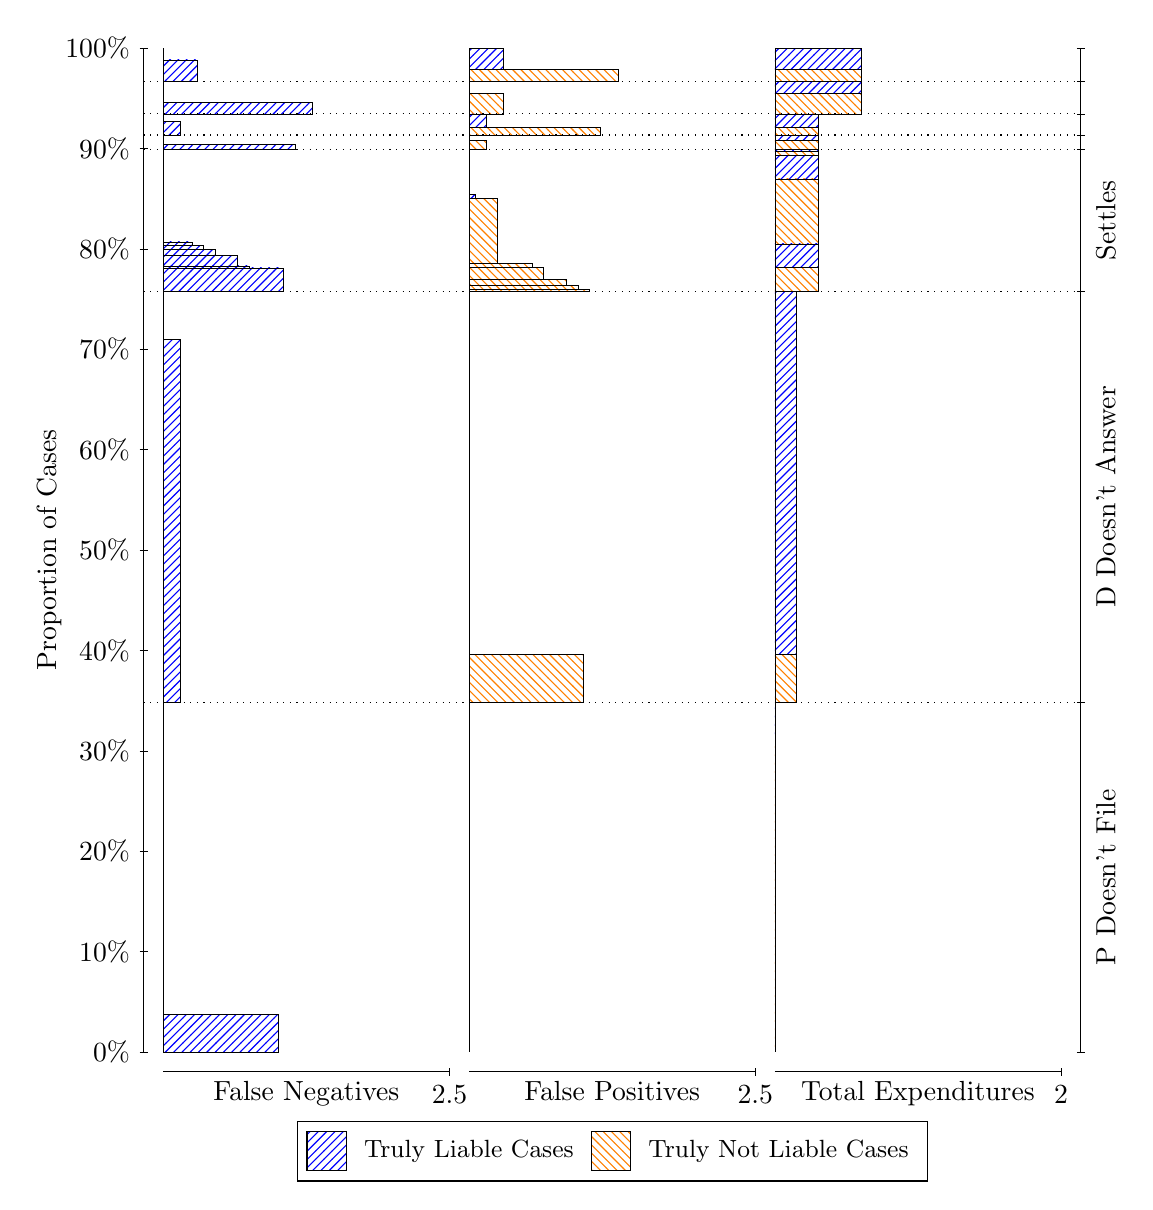
\begin{tikzpicture}
\draw[black, very thin] (1.5,1.75) -- (1.5,14.5);
\node[rotate=90, text=black, anchor=center] at (0.3, 8.125) {Proportion of Cases};
\draw[black, very thin] (1.45,1.75) -- (1.55,1.75);
\node[text=black, anchor=east] at (1.45, 1.75) {0\%};
\draw[black, very thin] (1.45,3.025) -- (1.55,3.025);
\node[text=black, anchor=east] at (1.45, 3.025) {10\%};
\draw[black, very thin] (1.45,4.3) -- (1.55,4.3);
\node[text=black, anchor=east] at (1.45, 4.3) {20\%};
\draw[black, very thin] (1.45,5.575) -- (1.55,5.575);
\node[text=black, anchor=east] at (1.45, 5.575) {30\%};
\draw[black, very thin] (1.45,6.85) -- (1.55,6.85);
\node[text=black, anchor=east] at (1.45, 6.85) {40\%};
\draw[black, very thin] (1.45,8.125) -- (1.55,8.125);
\node[text=black, anchor=east] at (1.45, 8.125) {50\%};
\draw[black, very thin] (1.45,9.4) -- (1.55,9.4);
\node[text=black, anchor=east] at (1.45, 9.4) {60\%};
\draw[black, very thin] (1.45,10.675) -- (1.55,10.675);
\node[text=black, anchor=east] at (1.45, 10.675) {70\%};
\draw[black, very thin] (1.45,11.95) -- (1.55,11.95);
\node[text=black, anchor=east] at (1.45, 11.95) {80\%};
\draw[black, very thin] (1.45,13.225) -- (1.55,13.225);
\node[text=black, anchor=east] at (1.45, 13.225) {90\%};
\draw[black, very thin] (1.45,14.5) -- (1.55,14.5);
\node[text=black, anchor=east] at (1.45, 14.5) {100\%};

\draw[black, very thin] (13.4,1.75) -- (13.4,14.5);
\draw[black, very thin] (13.35,1.75) -- (13.45,1.75);
\node[anchor=west] at (13.35, 1.75) {};
\draw[black, very thin] (13.35,6.1908) -- (13.45,6.1908);
\node[anchor=west] at (13.35, 6.1908) {};
\draw[black, very thin] (13.35,11.411) -- (13.45,11.411);
\node[anchor=west] at (13.35, 11.411) {};
\draw[black, very thin] (13.35,13.215) -- (13.45,13.215);
\node[anchor=west] at (13.35, 13.215) {};
\draw[black, very thin] (13.35,13.395) -- (13.45,13.395);
\node[anchor=west] at (13.35, 13.395) {};
\draw[black, very thin] (13.35,13.665) -- (13.45,13.665);
\node[anchor=west] at (13.35, 13.665) {};
\draw[black, very thin] (13.35,14.074) -- (13.45,14.074);
\node[anchor=west] at (13.35, 14.074) {};
\draw[black, very thin] (13.35,14.5) -- (13.45,14.5);
\node[anchor=west] at (13.35, 14.5) {};

\draw[black, very thin, pattern color=blue, pattern=north east lines] (1.75,1.75) rectangle (3.2033,2.2299);
\draw[black, very thin, pattern color=orange, pattern=north west lines] (1.75,2.2299) rectangle (1.75,6.1908);
\draw[black, very thin, pattern color=blue, pattern=north east lines] (1.75,6.1908) rectangle (1.968,10.798);
\draw[black, very thin, pattern color=orange, pattern=north west lines] (1.75,10.798) rectangle (1.75,11.411);
\draw[black, very thin, pattern color=blue, pattern=north east lines] (1.75,11.411) rectangle (3.276,11.708);
\draw[black, very thin, pattern color=blue, pattern=north east lines] (1.75,11.708) rectangle (2.84,11.734);
\draw[black, very thin, pattern color=blue, pattern=north east lines] (1.75,11.734) rectangle (2.6947,11.869);
\draw[black, very thin, pattern color=blue, pattern=north east lines] (1.75,11.869) rectangle (2.404,11.945);
\draw[black, very thin, pattern color=blue, pattern=north east lines] (1.75,11.945) rectangle (2.2587,11.989);
\draw[black, very thin, pattern color=blue, pattern=north east lines] (1.75,11.989) rectangle (2.1133,12.038);
\draw[black, very thin, pattern color=orange, pattern=north west lines] (1.75,12.038) rectangle (1.75,13.215);
\draw[black, very thin, pattern color=blue, pattern=north east lines] (1.75,13.215) rectangle (3.4213,13.28);
\draw[black, very thin, pattern color=orange, pattern=north west lines] (1.75,13.28) rectangle (1.75,13.395);
\draw[black, very thin, pattern color=blue, pattern=north east lines] (1.75,13.395) rectangle (1.968,13.567);
\draw[black, very thin, pattern color=orange, pattern=north west lines] (1.75,13.567) rectangle (1.75,13.665);
\draw[black, very thin, pattern color=blue, pattern=north east lines] (1.75,13.665) rectangle (3.6393,13.814);
\draw[black, very thin, pattern color=orange, pattern=north west lines] (1.75,13.814) rectangle (1.75,14.074);
\draw[black, very thin, pattern color=blue, pattern=north east lines] (1.75,14.074) rectangle (2.186,14.349);
\draw[black, very thin, pattern color=orange, pattern=north west lines] (1.75,14.349) rectangle (1.75,14.5);
\draw[black, very thin, pattern color=orange, pattern=north west lines] (5.6333,1.75) rectangle (5.6333,5.7109);
\draw[black, very thin, pattern color=blue, pattern=north east lines] (5.6333,5.7109) rectangle (5.6333,6.1908);
\draw[black, very thin, pattern color=orange, pattern=north west lines] (5.6333,6.1908) rectangle (7.0867,6.8033);
\draw[black, very thin, pattern color=blue, pattern=north east lines] (5.6333,6.8033) rectangle (5.6333,11.411);
\draw[black, very thin, pattern color=orange, pattern=north west lines] (5.6333,11.411) rectangle (7.1593,11.438);
\draw[black, very thin, pattern color=orange, pattern=north west lines] (5.6333,11.438) rectangle (7.014,11.482);
\draw[black, very thin, pattern color=orange, pattern=north west lines] (5.6333,11.482) rectangle (6.8687,11.558);
\draw[black, very thin, pattern color=orange, pattern=north west lines] (5.6333,11.558) rectangle (6.578,11.71);
\draw[black, very thin, pattern color=orange, pattern=north west lines] (5.6333,11.71) rectangle (6.4327,11.764);
\draw[black, very thin, pattern color=orange, pattern=north west lines] (5.6333,11.764) rectangle (5.9967,12.588);
\draw[black, very thin, pattern color=blue, pattern=north east lines] (5.6333,12.588) rectangle (5.706,12.637);
\draw[black, very thin, pattern color=blue, pattern=north east lines] (5.6333,12.637) rectangle (5.6333,13.215);
\draw[black, very thin, pattern color=orange, pattern=north west lines] (5.6333,13.215) rectangle (5.8513,13.33);
\draw[black, very thin, pattern color=blue, pattern=north east lines] (5.6333,13.33) rectangle (5.6333,13.395);
\draw[black, very thin, pattern color=orange, pattern=north west lines] (5.6333,13.395) rectangle (7.3047,13.492);
\draw[black, very thin, pattern color=blue, pattern=north east lines] (5.6333,13.492) rectangle (5.8513,13.665);
\draw[black, very thin, pattern color=orange, pattern=north west lines] (5.6333,13.665) rectangle (6.0693,13.925);
\draw[black, very thin, pattern color=blue, pattern=north east lines] (5.6333,13.925) rectangle (5.6333,14.074);
\draw[black, very thin, pattern color=orange, pattern=north west lines] (5.6333,14.074) rectangle (7.5227,14.225);
\draw[black, very thin, pattern color=blue, pattern=north east lines] (5.6333,14.225) rectangle (6.0693,14.5);
\draw[black, very thin, pattern color=orange, pattern=north west lines] (9.5167,1.75) rectangle (9.5167,5.7109);
\draw[black, very thin, pattern color=blue, pattern=north east lines] (9.5167,5.7109) rectangle (9.5167,6.1908);
\draw[black, very thin, pattern color=orange, pattern=north west lines] (9.5167,6.1908) rectangle (9.7892,6.8033);
\draw[black, very thin, pattern color=blue, pattern=north east lines] (9.5167,6.8033) rectangle (9.7892,11.411);
\draw[black, very thin, pattern color=orange, pattern=north west lines] (9.5167,11.411) rectangle (10.062,11.71);
\draw[black, very thin, pattern color=blue, pattern=north east lines] (9.5167,11.71) rectangle (10.062,12.014);
\draw[black, very thin, pattern color=orange, pattern=north west lines] (9.5167,12.014) rectangle (10.062,12.837);
\draw[black, very thin, pattern color=blue, pattern=north east lines] (9.5167,12.837) rectangle (10.062,13.134);
\draw[black, very thin, pattern color=orange, pattern=north west lines] (9.5167,13.134) rectangle (10.062,13.189);
\draw[black, very thin, pattern color=blue, pattern=north east lines] (9.5167,13.189) rectangle (10.062,13.215);
\draw[black, very thin, pattern color=orange, pattern=north west lines] (9.5167,13.215) rectangle (10.062,13.33);
\draw[black, very thin, pattern color=blue, pattern=north east lines] (9.5167,13.33) rectangle (10.062,13.395);
\draw[black, very thin, pattern color=orange, pattern=north west lines] (9.5167,13.395) rectangle (10.062,13.492);
\draw[black, very thin, pattern color=blue, pattern=north east lines] (9.5167,13.492) rectangle (10.062,13.665);
\draw[black, very thin, pattern color=orange, pattern=north west lines] (9.5167,13.665) rectangle (10.607,13.925);
\draw[black, very thin, pattern color=blue, pattern=north east lines] (9.5167,13.925) rectangle (10.607,14.074);
\draw[black, very thin, pattern color=orange, pattern=north west lines] (9.5167,14.074) rectangle (10.607,14.225);
\draw[black, very thin, pattern color=blue, pattern=north east lines] (9.5167,14.225) rectangle (10.607,14.5);
\draw[black, dotted] (1.5,6.1908) -- (13.4,6.1908);
\draw[black, dotted] (1.5,11.411) -- (13.4,11.411);
\draw[black, dotted] (1.5,13.215) -- (13.4,13.215);
\draw[black, dotted] (1.5,13.395) -- (13.4,13.395);
\draw[black, dotted] (1.5,13.665) -- (13.4,13.665);
\draw[black, dotted] (1.5,14.074) -- (13.4,14.074);
\draw[black, very thin] (1.75,1.5) -- (5.3833,1.5);
\node[text=black, anchor=north] at (3.5667, 1.5) {False Negatives};
\draw[black, very thin] (5.3833,1.45) -- (5.3833,1.55);
\node[text=black, anchor=north] at (5.3833, 1.45) {2.5};

\draw[black, very thin] (5.6333,1.5) -- (9.2667,1.5);
\node[text=black, anchor=north] at (7.45, 1.5) {False Positives};
\draw[black, very thin] (9.2667,1.45) -- (9.2667,1.55);
\node[text=black, anchor=north] at (9.2667, 1.45) {2.5};

\draw[black, very thin] (9.5167,1.5) -- (13.15,1.5);
\node[text=black, anchor=north] at (11.333, 1.5) {Total Expenditures};
\draw[black, very thin] (13.15,1.45) -- (13.15,1.55);
\node[text=black, anchor=north] at (13.15, 1.45) {2};

\node[text=black, centered, rotate=90] at (13.72, 3.9704) {P Doesn't File};
\node[text=black, centered, rotate=90] at (13.72, 8.8007) {D Doesn't Answer};
\node[text=black, centered, rotate=90] at (13.72, 12.313) {Settles};





\draw (7.449999999999999,1.5) node[draw=none] (baseCoordinate) {};
\begin{scope}[align=center]
        \matrix[scale=0.5, draw=black, below=0.5cm of baseCoordinate, nodes={draw}, column sep=0.1cm]{
            \node[rectangle, draw, minimum width=0.5cm, minimum height=0.5cm, pattern color=blue, pattern=north east lines] {}; &
            \node[draw=none, font=\small, text=black] (B) {Truly Liable Cases}; &
            \node[rectangle, draw, minimum width=0.5cm, minimum height=0.5cm, pattern color=orange, pattern=north west lines] {}; &
            \node[draw=none, font=\small, text=black] (B) {Truly Not Liable Cases}; \\
            };
\end{scope}

\end{tikzpicture}
\end{document}